\documentclass{beamer}

\usepackage[sfdefault]{cabin}
\usepackage[utf8]{inputenc}
\usepackage[T1]{fontenc}
\usepackage[french]{babel}
\usepackage{xcolor}
\usepackage{caption}
\usepackage{graphicx}
%Police
%\usepackage[sfdefault]{roboto}
\usepackage[sfdefault]{FiraSans}

\definecolor{modernblue}{RGB}{70,130,180} 
\definecolor{modernvert}{RGB}{0, 80, 0} 

\usetheme{Madrid}

\usecolortheme[named=modernblue]{structure}

\setbeamertemplate{caption}{\insertcaption} % Utiliser le format de légende par défaut de Beamer

\title{Application des séries chronologiques sur les données Dataset\_CB.csv}
\author{Youness et Ivanhoé}
\date{11 janvier 2024}

\renewcommand{\thesection}{\Roman{section}}\renewcommand{\thesubsection}{\arabic{subsection} }\renewcommand{\thesubsubsection}{\alph{subsubsection} }

\newcommand{\C}{\mathbb{C}}\newcommand{\R}{\mathbb{R}}\newcommand{\Q}{\mathbb{Q}}\newcommand{\Z}{\mathbb{Z}}\newcommand{\N}{\mathbb{N}}\newcommand{\V}{\overrightarrow}\newcommand{\Cs}{\mathscr{C}}\newcommand{\Ps}{\mathscr{P}}\newcommand{\Rs}{\mathscr{R}}\newcommand{\Gs}{\mathscr{G}}\newcommand{\Ds}{\mathscr{D}}\newcommand{\happy}{\huge\smiley}\newcommand{\sad}{\huge\frownie}\newcommand{\alors}{\Large\Rightarrow}\newcommand{\equi}{\Leftrightarrow}
\newcommand{\disp}{\displaystyle}\newcommand{\Pro}{\mathbb{P}}


\newtheorem{thm}{Théorème}
\newtheorem{rmq}{Remarque}
\newtheorem{prop}{Propriété}
\newtheorem{cor}{Corollaire}
\newtheorem{lem}{Lemme}
\newtheorem{prop-def}{Propriété-définition}

\theoremstyle{definition}

\newtheorem{defi}{Définition}
\newtheorem{intro}{Initialisation}
\newtheorem{boucle}{Boucle principale}
\newtheorem{ex}{Exemple}
\newtheorem*{rap}{Rappel}
\newtheorem{cex}{Contre-exemple}
\newtheorem{exer}{Exercice} % \large {\fontfamily{ptm}\selectfont EXERCICE}
\newtheorem{nota}{Notation}
\newtheorem{ax}{Axiome}
\newtheorem{appl}{Application}
\newtheorem{csq}{Conséquence}
\def\di{\displaystyle}



\begin{document}
\begin{frame}[plain]
    \maketitle
\end{frame}


\begin{frame}
\frametitle{Introduction}
\hfill\\[-0.75cm]
\begin{figure}
	\centering
	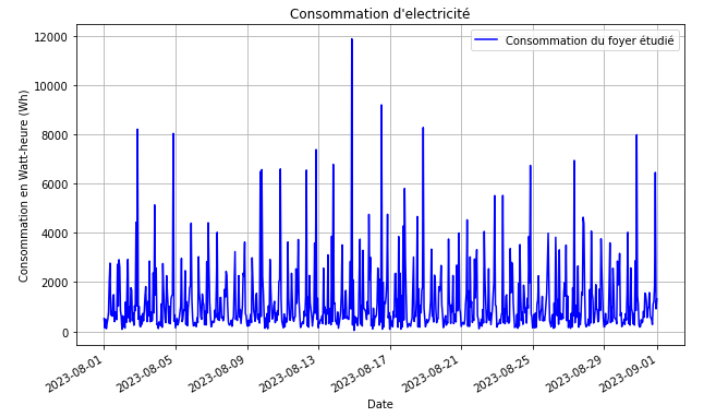
\includegraphics[scale=0.35]{1.png}\\[-0.25cm]
	\caption*{Voici un série chronologique issue de données pseudo-réelles issue d'une consommation EDF d'un foyer.}
\end{figure}

\textcolor{modernvert}{\textbf{Problématique :}} Comment prédire à horizon de 7 jours la
consommation électrique du foyer sur la première semaine de septembre 2023 ?
\end{frame}

\begin{frame}
	\tableofcontents
\end{frame}

\section{Partie preprocessing}
\begin{frame}
	\frametitle{Renommer les colonnes et passer au format date}
		\begin{minipage}[c]{1\linewidth}
		\begin{minipage}[c]{0.4\linewidth}\centering\begin{figure}
				\centering
				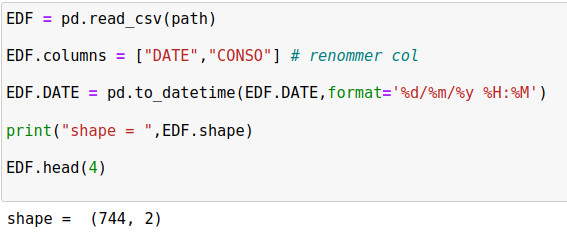
\includegraphics[scale=0.28]{2.png}
				\caption*{Chargement des données}
				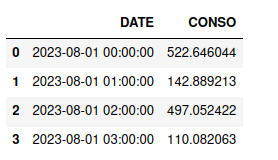
\includegraphics[width=1\linewidth]{3.png}
				\caption*{Dataset EDF}
		\end{figure}\end{minipage}\hfill 
		\begin{minipage}[c]{0.5\linewidth}\centering\begin{figure}
				\begin{center}
					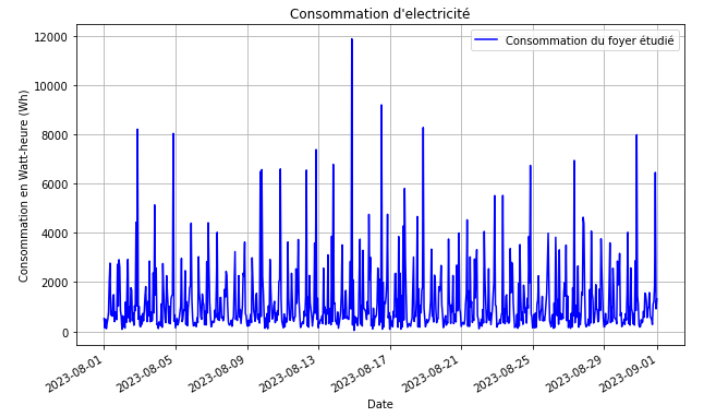
\includegraphics[width=1\linewidth]{1.png}			
					\caption*{Consommation du foyer}
				\end{center}
				
		\end{figure}\end{minipage}
	\end{minipage}	
\end{frame}

\begin{frame}
	\frametitle{Passage au log pour réduire la variabilité de la série}
	\begin{minipage}[c]{1\linewidth}
		\begin{minipage}[c]{0.4\linewidth}\centering\begin{figure}
				\centering
				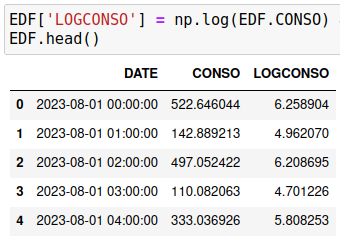
\includegraphics[width=1\linewidth]{4.png}
				\caption*{Dataset EDF}
		\end{figure}\end{minipage}\hfill 
		\begin{minipage}[c]{0.58\linewidth}\centering\begin{figure}
				\begin{center}
					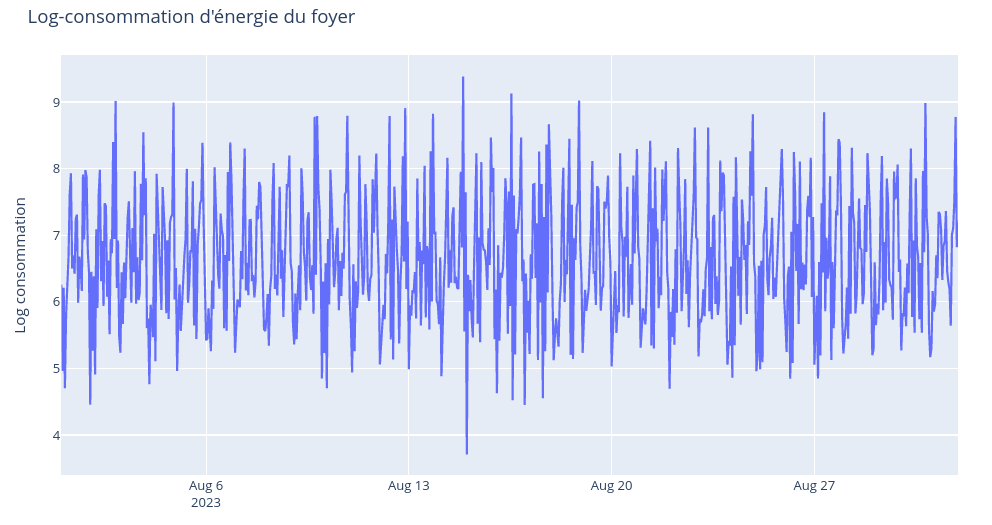
\includegraphics[width=1\linewidth]{5.png}			
					\caption*{Log-consommation du foyer}
				\end{center}
				
		\end{figure}\end{minipage}
	\end{minipage}
	
\end{frame}
\section{Stationnarité et vérification}
\begin{frame}
	\frametitle{Étude de la stationnarité de la log-consommation}
	\begin{minipage}[t]{1\linewidth}
	\begin{minipage}[c]{0.58\linewidth}\centering\begin{figure}
			\centering
			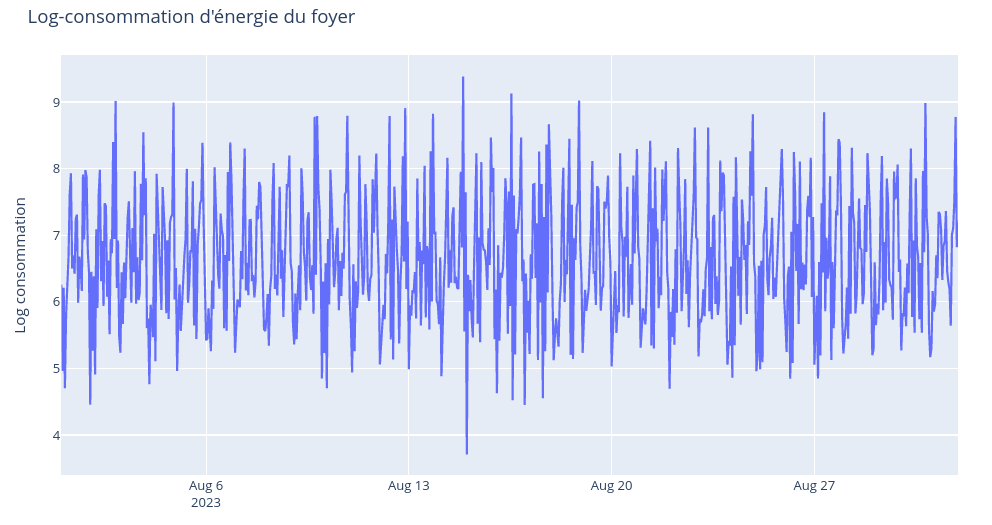
\includegraphics[width=1\linewidth]{5.png}
			\caption*{Log-consommation du foyer}
	\end{figure}\end{minipage}\hfill 
	\begin{minipage}[c]{0.4\linewidth}\centering\begin{figure}
			\begin{center}
				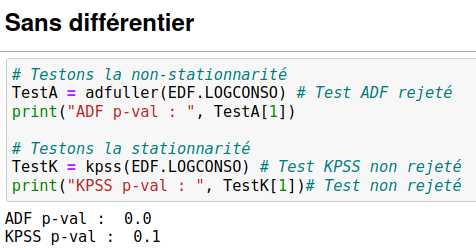
\includegraphics[width=1\linewidth]{6.png}			
				\caption*{Tests ADF et KPSS}
			\end{center}
			
	\end{figure}\end{minipage}
\end{minipage}
	
\end{frame}

\begin{frame}
	\frametitle{Étude de la stationnarité de la log-consommation avec une différentiation saisonnière}
	\begin{minipage}[t]{1\linewidth}
		\begin{minipage}[c]{0.55\linewidth}\centering\begin{figure}
				\centering
				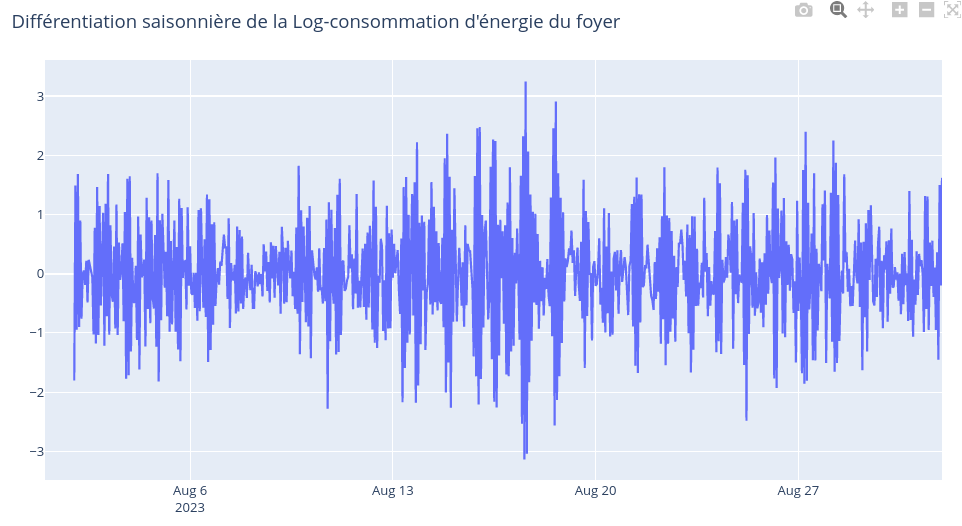
\includegraphics[width=1\linewidth]{8.png}
				\caption*{Différentielle saisonnière log-consommation du foyer}
		\end{figure}\end{minipage}\hfill 
		\begin{minipage}[c]{0.44\linewidth}\centering\begin{figure}
				\begin{center}
					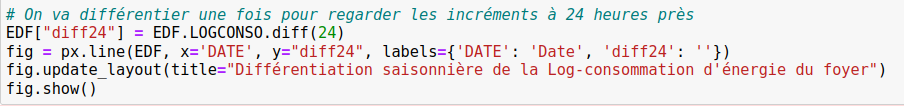
\includegraphics[width=1\linewidth]{7.png}
					\caption*{Différentiation D=24}
					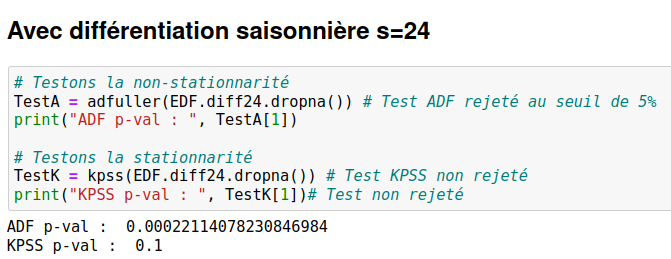
\includegraphics[width=1\linewidth]{9.png}			
					\caption*{Tests ADF et KPSS}
				\end{center}
				
		\end{figure}\end{minipage}
	\end{minipage}
	
\end{frame}

\section{Étude des corrélations}

\begin{frame}
	\frametitle{Étude des corrélations sur la série temporelle}
	\begin{minipage}[t]{1\linewidth}
		\centering
		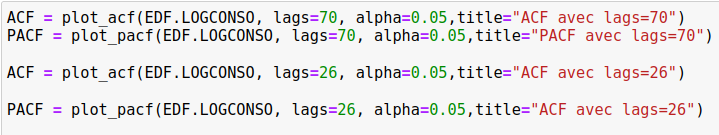
\includegraphics[width=0.8\linewidth]{10.png}
		\begin{minipage}[c]{0.48\linewidth}\centering\begin{figure}
				\centering
				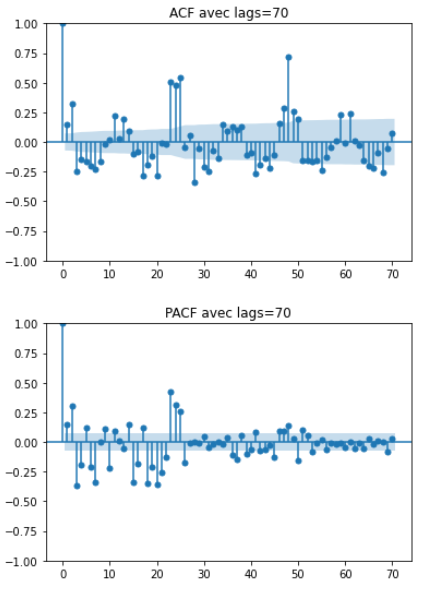
\includegraphics[width=0.75\linewidth]{11.png}	
		\end{figure}\end{minipage}\hfill 
		\begin{minipage}[c]{0.48\linewidth}\centering\begin{figure}
				\begin{center}
					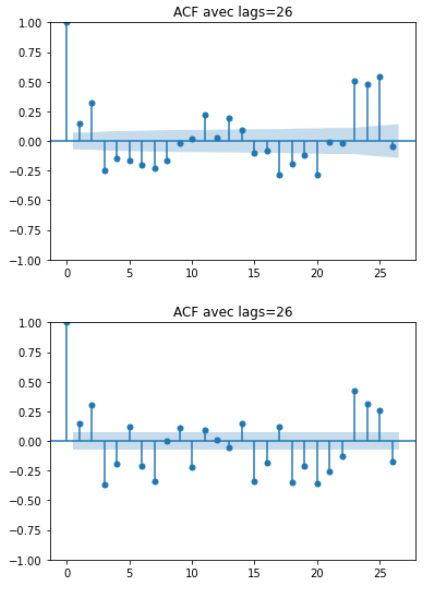
\includegraphics[width=0.75\linewidth]{12.png}			
				\end{center}
				
		\end{figure}\end{minipage}
	\end{minipage}
	
\end{frame}


\section{Recherche de modèles significatifs}
\section{Cross validation et évaluation}
\section{Prédiction avec le meilleur modèle}





\end{document}








